% This is samplepaper.tex, a sample chapter demonstrating the
% LLNCS macro package for Springer Computer Science proceedings;
% Version 2.21 of 2022/01/12
%
\documentclass[runningheads]{llncs}
%
\usepackage[T1]{fontenc}
% T1 fonts will be used to generate the final print and online PDFs,
% so please use T1 fonts in your manuscript whenever possible.
% Other font encondings may result in incorrect characters.


% tightlist command for lists without linebreak
\providecommand{\tightlist}{%
  \setlength{\itemsep}{0pt}\setlength{\parskip}{0pt}}


% Pandoc citation processing
\newlength{\cslhangindent}
\setlength{\cslhangindent}{1.5em}
\newlength{\csllabelwidth}
\setlength{\csllabelwidth}{3em}
\newlength{\cslentryspacingunit} % times entry-spacing
\setlength{\cslentryspacingunit}{\parskip}
% for Pandoc 2.8 to 2.10.1
\newenvironment{cslreferences}%
  {}%
  {\par}
% For Pandoc 2.11+
\newenvironment{CSLReferences}[2] % #1 hanging-ident, #2 entry spacing
 {% don't indent paragraphs
  \setlength{\parindent}{0pt}
  % turn on hanging indent if param 1 is 1
  \ifodd #1
  \let\oldpar\par
  \def\par{\hangindent=\cslhangindent\oldpar}
  \fi
  % set entry spacing
  \setlength{\parskip}{#2\cslentryspacingunit}
 }%
 {}
\usepackage{calc}
\newcommand{\CSLBlock}[1]{#1\hfill\break}
\newcommand{\CSLLeftMargin}[1]{\parbox[t]{\csllabelwidth}{#1}}
\newcommand{\CSLRightInline}[1]{\parbox[t]{\linewidth - \csllabelwidth}{#1}\break}
\newcommand{\CSLIndent}[1]{\hspace{\cslhangindent}#1}

\usepackage[hidelinks]{hyperref}


\usepackage{graphicx}
% Used for displaying a sample figure. If possible, figure files should
% be included in EPS format.
%
% If you use the hyperref package, please uncomment the following two lines
% to display URLs in blue roman font according to Springer's eBook style:
\usepackage{hyperref}
\usepackage{color}
\renewcommand\UrlFont{\color{blue}\rmfamily}


\begin{document}


\title{Estimating the socio-environmental impacts of car substitution by
bicycle and public transit using open tools}
%
\titlerunning{Estimating the SE impacts of car substitution by bicycle
and public transit}
% If the paper title is too long for the running head, you can set
% an abbreviated paper title here
%
\author{Rosa Félix\inst{1}\orcidID{0000-0002-5642-6006} \and Filipe
Moura\inst{1}\orcidID{0000-0001-7749-8490} \and Robin
Lovelace\inst{2}\orcidID{0000-0001-5679-6536}}


\authorrunning{R. Félix et al.}
% First names are abbreviated in the running head.
% If there are more than two authors, 'et al.' is used.
%

\institute{CERIS - Instituto Superior Técnico, University of Lisbon. Av
Rovisco Pais 1049-001 Lisboa, Portugal\\
\email{\href{mailto:rosamfelix@tecnico.ulisboa.pt}{\nolinkurl{rosamfelix@tecnico.ulisboa.pt}}}\\ \and Institute
for Transport Studies, University of Leeds. 34-40 University Rd, Leeds
LS2 9JT, UK}

\maketitle              % typeset the header of the contribution
%
\begin{abstract}
In metropolitan areas, car trips can be replaced by a combination of
public transit and cycling for the first-and-last mile. This paper
focuses on estimating the potential for cycling + PT as a substitute for
car trips in the Lisbon metropolitan area and assessing its
socio-environmental impacts using open data and open source tools. A
decision support tool that facilitates the design and development of a
metropolitan cycling network was developed (\emph{biclaR}). A scenario
of intermodality introduced, and its socio-environmental impacts were
assessed using the \emph{HEAT for Cycling} and the \emph{HEAT as a
Service} tools. Additionally, the impacts of shifting car trips to PT
were estimated and monetized. The results indicate that 20\% of the
current trips can be made with the bicycle + PT combination. Shifting to
cycling for the first-and-last mile can reduce annual CO2eq emissions
from 6,000 tons/day, and the 10-year socio-environmental benefits
account from €230 million. For the PT leg, the transfer from car results
in the avoidance of at lest 8,500 tons of CO2eq emissions per year. The
information on socio-economic benefits can support policymakers in
prioritizing interventions to reduce the reliance on individual
motorized transportation and effectively communicate their decisions.

\keywords{Active transport \and Intermodality \and First and last
mile \and Health economic assessment \and Environmental
impacts \and Open data and methods}

\end{abstract}

\hypertarget{introduction}{%
\section{Introduction}\label{introduction}}

In metropolitan areas, car trips can be replaced by a combination of
public transit (PT) and cycling for the first-and-last mile. This
approach requires interventions and programs to make bicycling more
appealing, and the resulting public investments can have significant
social and environmental benefits. This paper focuses on estimating the
potential for cycling + PT as a substitute for car trips in the Lisbon
metropolitan area (LMA) and assessing its socio-environmental impacts
using open data and open source tools.

According to the latest mobility survey conducted in 2018, the LMA
registered a total of 5.3 million daily trips, with only 0.5\% by
bicycle. Car modal share is 58.4\%, while PT accounts for 15.5\%. To
achieve the cycling targets set by the Portuguese national cycling
strategy for 2025 and 2030 (4\% and 10\%, respectively), the Department
of Transport introduced biclaR, a decision support tool that facilitates
the design and development of a metropolitan cycling network.

This research aims to present and discuss the methods used to
estimate\ldots{}

Propensity to Cycle Tool

adding up an intermodality scenario to estimate cycling potential to
public transit interfaces, and thus to support planning and prioritize
investments in the cycling network.

\hypertarget{methods}{%
\section{Methods}\label{methods}}

\hypertarget{case-study}{%
\subsection{Case Study}\label{case-study}}

\hypertarget{modeling-origin-destination-trips}{%
\subsection{Modeling Origin-Destination
trips}\label{modeling-origin-destination-trips}}

\hypertarget{modeling-intermodality}{%
\subsection{Modeling intermodality}\label{modeling-intermodality}}

The intermodality scenario considers trips that can combine PT and
cycling for the first-and-last legs. Conservatively, we considered the
sum of first-and-last legs up to 5 km. Furthermore, we restricted PT use
to unimodal trips without transfers (although they can be included in
future modeling). Félix, Lovelace, and Moura (2022)

Finally, we only included PT modes that can practically accommodate
bicycles, such as trains, ferries, trams, and intermunicipal bus lines
with bike racks (~\ref{fig:map1}).

\begin{figure}
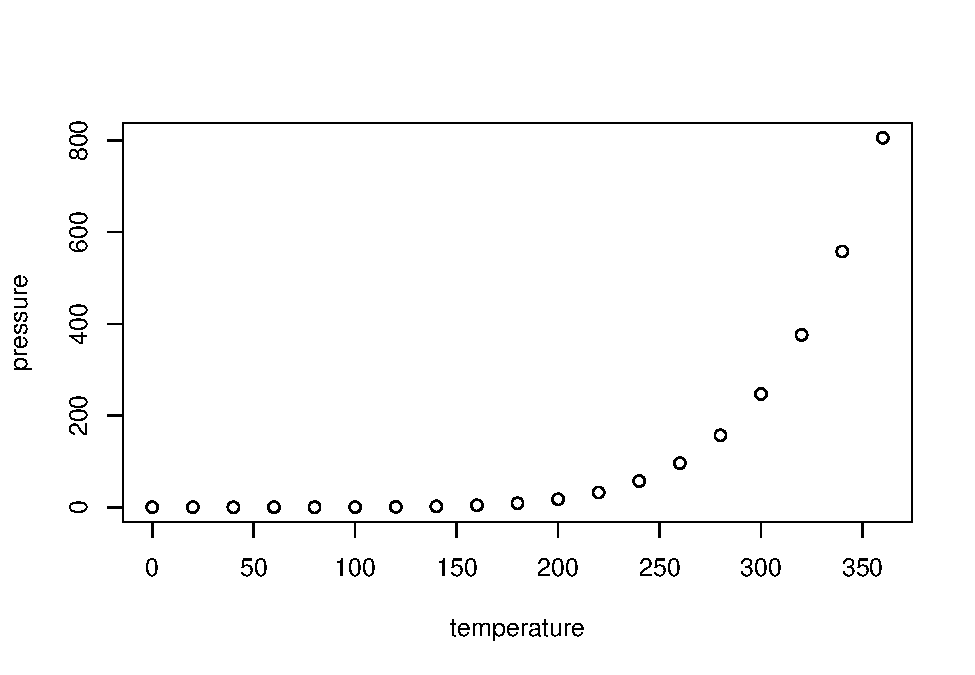
\includegraphics{PaperTRA_files/figure-latex/map1-1} \caption{Interfaces and lines considered, by transport mode, in the Lisbon metropolitan area}\label{fig:map1}
\end{figure}

To obtain reliable results, we used the OpenStreetMap road network and
GTFS data. The r5r R package estimated the trip duration and distance
for both the original modes and the bicycle + PT combination, while the
od jittering R package estimated the OD locations based on a
centroid-based OD matrix.

\hypertarget{assessing-socio-environmental-benefits}{%
\subsection{Assessing socio-environmental
benefits}\label{assessing-socio-environmental-benefits}}

Socio-environmental impacts were assessed using the HEAT for Cycling and
the HEAT as a Service tools, from the WHO. Additionally, we estimate the
impacts of shifting car trips to PT for the second leg of the journey
with EMEP/EEA's COPERT methodology and monetize them with the EU Guide
to cost-benefit analysis.

Table~\ref{tab:table} gives a summary of all heading levels.

\begin{table}

\caption{\label{tab:table}Table captions should be placed above the tables.}
\centering
\begin{tabular}[t]{r|r}
\hline
temperature & pressure\\
\hline
0 & 0.0002\\
\hline
20 & 0.0012\\
\hline
40 & 0.0060\\
\hline
60 & 0.0300\\
\hline
80 & 0.0900\\
\hline
100 & 0.2700\\
\hline
\end{tabular}
\end{table}

\hypertarget{results-and-discussion}{%
\section{Results and Discussion}\label{results-and-discussion}}

The results indicate that 20\% of the current trips can be made with the
bicycle + PT combination, with an additional 12\% of PT trips being
potentially replaced. Shifting to cycling for the first-and-last mile
can reduce annual CO2eq emissions by 6,000 to 15,000 tons/day, and the
10-year socio-environmental benefits account for €230 to €590 million,
depending on the cycling targets. For the PT leg, the transfer from car
results in the avoidance of 8,500 to 20,800 tons of CO2eq emissions per
year, or €1.4 to €3.5 million over 10 years, with trains offering the
greatest potential for substitution (88\%).

Map result (~\ref{fig:map2}).

\begin{figure}
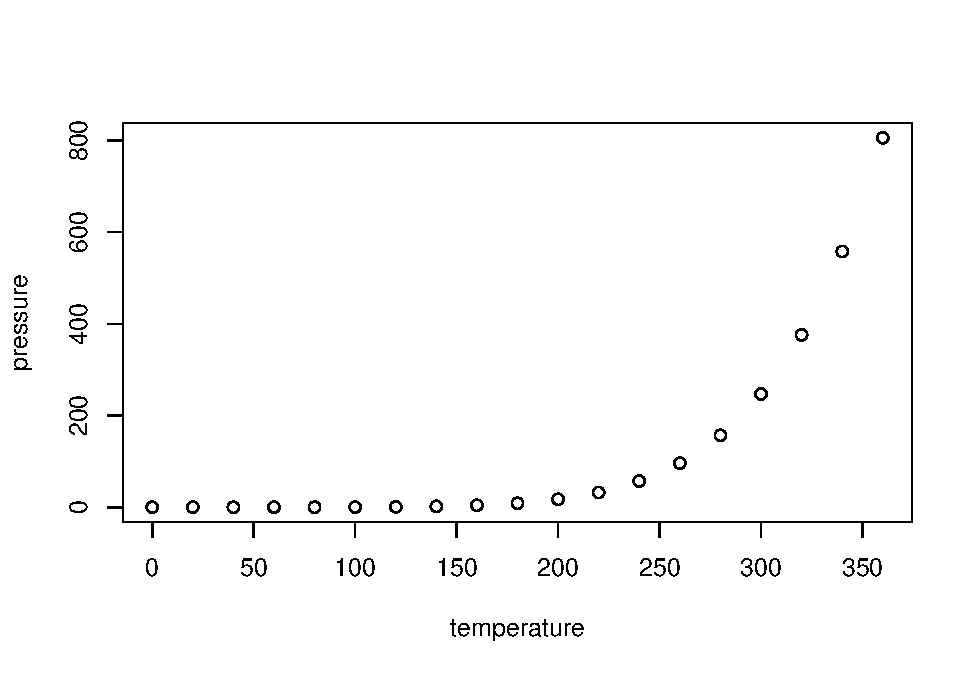
\includegraphics{PaperTRA_files/figure-latex/map2-1} \caption{Bike routes with highest potential to serve as first and last mile when replacing cycling and PT from car trips (screenshot of the interactive online tool).}\label{fig:map2}
\end{figure}

\hypertarget{conclusion}{%
\section{Conclusion}\label{conclusion}}

By making the research process publicly accessible in a code repository,
this study enables the replication of similar estimates for
socio-environmental impacts resulting from a modal shift from cars to
bicycles + PT in other metropolitan areas. The provided information on
socio-economic benefits can support policymakers in prioritizing
interventions to reduce the reliance on individual motorized
transportation and effectively communicate their decisions.

\hypertarget{acknowledgements}{%
\subsubsection*{Acknowledgements}\label{acknowledgements}}
\addcontentsline{toc}{subsubsection}{Acknowledgements}

Please place your acknowledgments at the end of the paper, preceded by
an unnumbered run-in heading (i.e.~3rd-level heading).

Thomas Götshi - HAAS.

\hypertarget{references}{%
\section*{References}\label{references}}
\addcontentsline{toc}{section}{References}

\hypertarget{refs}{}
\begin{CSLReferences}{1}{0}
\leavevmode\vadjust pre{\hypertarget{ref-felix2023}{}}%
Félix, Rosa, Robin Lovelace, and Filipe Moura. 2022. {``{biclaR -
Ferramenta de apoio ao planeamento da rede ciclável na área
metropolitana de Lisboa}.''} {CERIS - Instituto Superior Técnico and
Transportes Metropolitanos de Lisboa}.
\url{https://biclar.tmlmobilidade.pt}.

\leavevmode\vadjust pre{\hypertarget{ref-bib2}{}}%
Slifka, M. K., and J. L. Whitton. 2000. {``Clinical Implications of
Dysregulated Cytokine Production.''} \emph{J. {M}ol. {M}ed.} 78: 74--80.
\url{https://doi.org/10.1007/s001090000086}.

\end{CSLReferences}

%
% ---- Bibliography ----



\end{document}
